\documentclass[10pt]{beamer}

\usepackage{appendixnumberbeamer}
\usepackage{booktabs}
\usepackage[scale=2]{ccicons}
\usepackage{pgfplots}
\usepackage{graphics}
\usepackage{braket}

\usepgfplotslibrary{dateplot}
\pdfstringdefDisableCommands{\def\translate#1{#1}}
\geometry{paperwidth=140mm, paperheight=105mm}
\usetheme{metropolis}
\bibliographystyle{abbrv}
\setbeamertemplate{frame footer}{ME738 - Special Topics in Materials}

\renewcommand{\footnotesize}{\fontsize{7pt}{8pt}\selectfont}

\title{Chip Scale Atomic Clocks Sources}
\subtitle{Working principles}
\date{March 20, 2024}
\author{Tommaso Bocchietti}
\institute{University of Waterloo}
\titlegraphic{\hfill\includegraphics[height=1.5cm]{pdf/UniversityOfWaterloo_logo_horiz_pms.pdf}}

\begin{document}

\maketitle

\include{src/01-toolbox}
\section{CSAC Block Diagram}

\begin{frame}{Block diagram of a generic CSAC}

    \begin{figure}
        \centering
        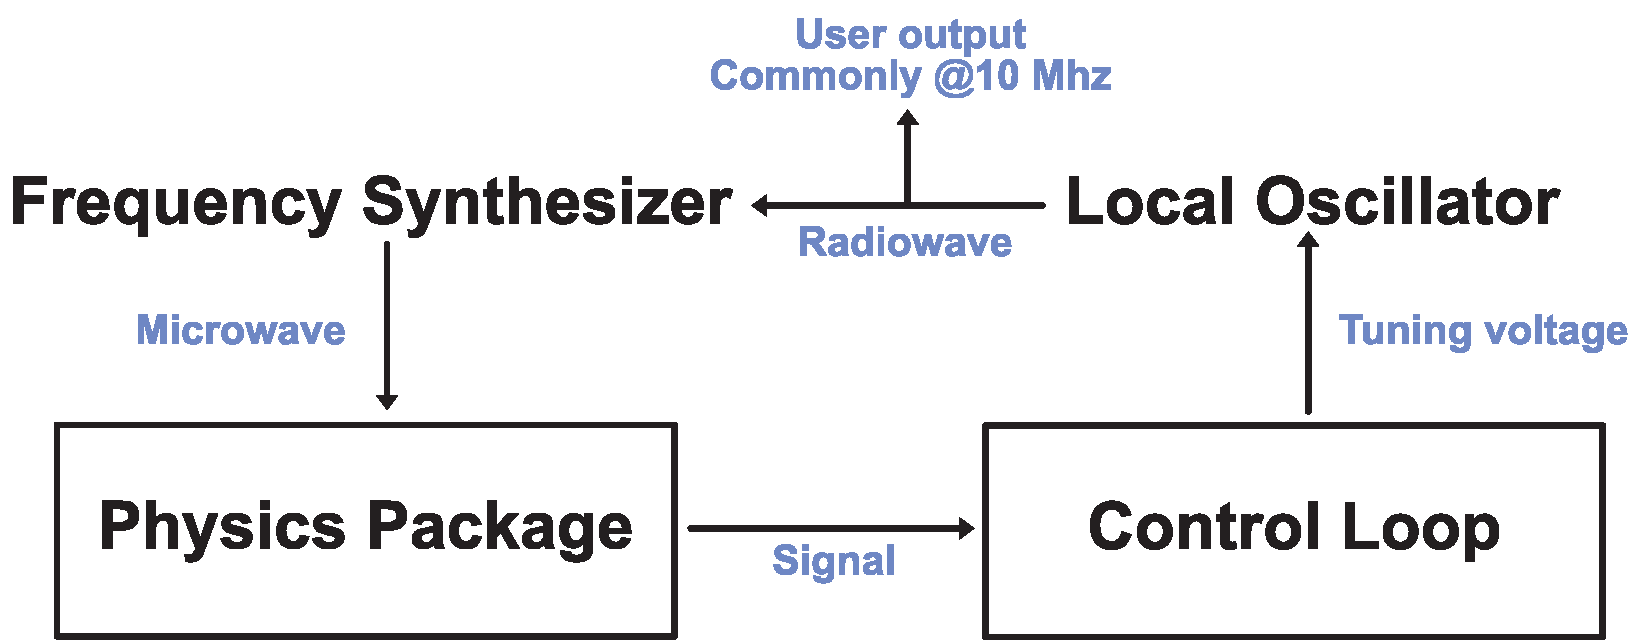
\includegraphics[width=0.8\textwidth]{pdf/CSAC-block-diagram.pdf}
    \end{figure}

    In the following slides, we are going to see:

    \begin{itemize}
        \item Physics Package
              \begin{itemize}
                  \item Based on Microwave Optical Double-Resonance (MODR)
                  \item Based on Coherent Population Trapping (CPT)
              \end{itemize}
        \item Control loop
        \item Local Oscillator
    \end{itemize}

\end{frame}
\section{Physics Package based on Microwave Optical Double-Resonance (MODR)}

\begin{frame}{$^{87}Rb$ Reference Cell}

    At the heart of a MODR based CSAC, we find a $^{87}Rb$ reference cell.

    \vspace{10pt}

    \begin{columns}[c, onlytextwidth]

        \begin{column}{0.45\textwidth}

            \begin{figure}
                \centering
                \only<1>{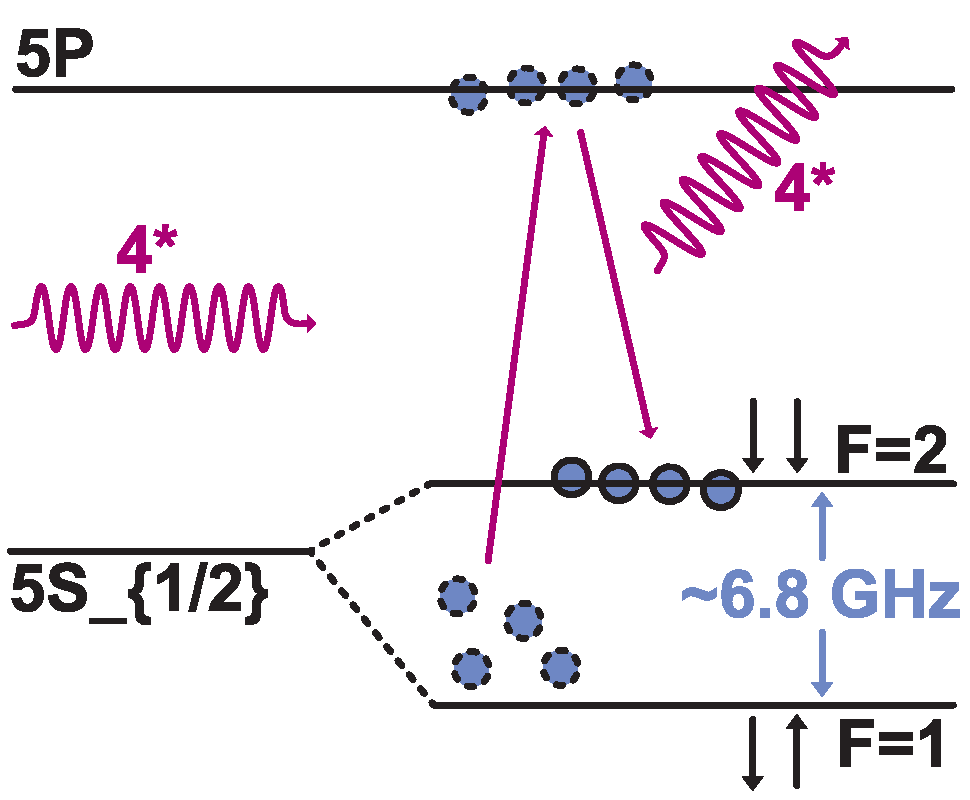
\includegraphics[width=0.9\textwidth]{pdf/MODR/pumping-decay.pdf}}
                \only<2>{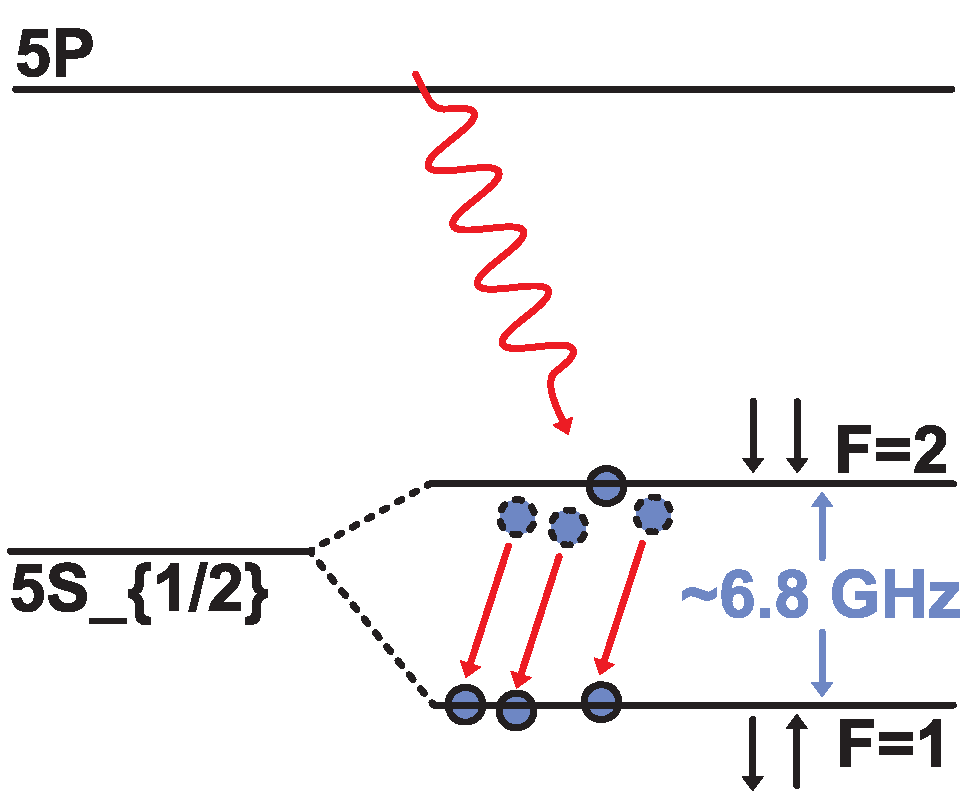
\includegraphics[width=0.9\textwidth]{pdf/MODR/microwave.pdf}}
                \only<3>{\includegraphics[width=0.9\textwidth]{pdf/MODR/interrogation.pdf}}
            \end{figure}

        \end{column}

        \begin{column}{0.55\textwidth}

            We can distinguish 3 processes:

            \begin{enumerate}
                \item<1-> \textbf<1>{Optical Pumping (Population Inversion)}
                \item<2-> \textbf<2>{Microwave Excitation}
                \item<3-> \textbf<3>{Optical Pumping (Interrogation)}
            \end{enumerate}

        \end{column}

    \end{columns}

    \vspace{10pt}

    \only<1>{
        Ground state population $F=\ket{1}$ gets pumped to $5P$ and then decay to both $F=\ket{1}$ \& $F=\ket{2}$.

        Over time, the population will accumulate in the $F=\ket{2}$ state.
    }
    \only<2>{Microwave tuned at the atomic resonance frequency ($\approx 6.8$ GHz) brings part of the population back to $F=\ket{1}$.}
    \only<3>{Depending on the intensity of the transmitted radiation, \textbf{we can infer if the microwave frequency was in resonance or not}.}

\end{frame}



\begin{frame}{Photodetection}

    At the end of the cell, a photodiode is used to measure the intensity of the transmitted radiation.

    \begin{figure}
        \centering
        \includegraphics[width=0.7\textwidth]{img/MODR-transmission-curve.jpg}
    \end{figure}

    Our target is to stay at the dip of the transmission curve.

\end{frame}



\begin{frame}{Complete Physics Package for a MODR-based CSAC}

    % Previously analyzed components: \textit{Absorption Cell} and \textit{Photocell}.

    \begin{figure}
        \centering
        \includegraphics[width=0.7\textwidth]{img/MODR-physics-package.png}
    \end{figure}

    Other notable components are:

    \begin{itemize}
        \item $^{87}Rb$ Bulb: high frequency radiation source.
        \item $^{85}Rb$ Filter cell: because of overlapping hyperfine levels, it filters out the unwanted transitions frequencies from the lamp.
        \item Microwave cavity: enhances the interaction between radiation and atoms.
    \end{itemize}

\end{frame}


\begin{frame}{Design bottleneck}

    \textit{\dots goal of developing an ultra-miniaturized, low-power, atomic time and frequency reference units\dots}

    \vspace{10pt}

    In case of a MODR-based CSAC, we can recognize multiple problematic areas:

    \begin{itemize}
        \item \textbf{Size}: microwave cavity imposes a low limit ($L_{min} = \frac{c}{2f_{transition}} \approx 2.2cm$).
        \item \textbf{Power consumption}: high ($\approx 10W$) due to thermal stabilization ($\approx 70\%$ of the total).
        \item \textbf{Optical instabilities}: internal wall gas collision\footnotemark[1], Zeeman effects\footnotemark[1], Stark shifts.
    \end{itemize}

    \footnotetext[1]{More on this in the "Extra slides" section.}

\end{frame}


% \begin{frame}{Microwave Cavity}
%     The microwave cavity is used to enhance the interaction between the microwave radiation and the atoms.
%     The cavity is tuned to the atomic resonance frequency.
% \end{frame}
\section{Physics Package based on Coherent Population Trapping (CPT)}
% CPT (Coherent Population Trapping) (theory -> physical components -> VCSEL

\begin{frame}{Superposition of Quantum States (concept)}

    Before exploring the CPT itself, it's important to understand the concept of superposition of quantum states by using the Bloch sphere representation.

    \begin{columns}

        \begin{column}{0.32\textwidth}

            \onslide<2->{
                \begin{figure}
                    \centering
                    \includegraphics[width=0.9\textwidth]{pdf/states/ground-state.pdf}
                    \caption{Ground state}
                \end{figure}
            }

        \end{column}

        \begin{column}{0.32\textwidth}

            \onslide<4->{
                \begin{figure}
                    \centering
                    \includegraphics[width=0.9\textwidth]{pdf/states/superposition-state.pdf}
                    \caption{Superposition of states}
                \end{figure}
            }

        \end{column}

        \begin{column}{0.32\textwidth}

            \onslide<3->{
                \begin{figure}
                    \centering
                    \includegraphics[width=0.9\textwidth]{pdf/states/excited-state.pdf}
                    \caption{Excited state}
                \end{figure}
            }

        \end{column}

    \end{columns}

    \onslide<3->{
        \begin{figure}

            \centering

            \resizebox{\columnwidth}{!}{%
                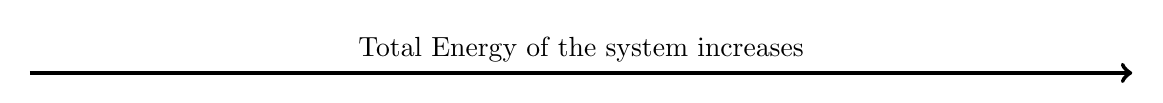
\begin{tikzpicture}[scale=0.5]
                    \draw[ultra thick, ->] (0,0) -> (28,0) node[midway, above] {Total Energy of the system increases};
                \end{tikzpicture}
            }

        \end{figure}
    }

\end{frame}



\begin{frame}{Dark state \& $\Lambda$-system}

    \textit{"In atomic physics, a dark state refers to a state of an atom or molecule that cannot absorb (or emit) photons."}

    \begin{columns}[T, onlytextwidth]

        \begin{column}{0.45\textwidth}

            \begin{figure}
                \centering
                \includegraphics[width=\textwidth]{pdf/lambda-system.pdf}
                \caption{$\Lambda$-system.}
            \end{figure}

        \end{column}

        \begin{column}{0.55\textwidth}

            \vspace{30pt}

            \begin{align}
                \text{Allowed transitions:}  & \begin{cases}
                                                   \ket{1} \leftrightarrow \ket{3} \\
                                                   \ket{2} \leftrightarrow \ket{3}
                                               \end{cases} \\
                \text{Forbidden transition:} & \begin{cases}
                                                   \ket{1} \leftrightarrow \ket{2}
                                               \end{cases}
            \end{align}

        \end{column}

    \end{columns}

    \vspace{10pt}

    In this case the dark state happens to be a superposition of $\ket{1}$ and $\ket{2}$.

\end{frame}



\begin{frame}{$^{133}Cs$ Reference Cell}

    At the heart of a CPT based CSAC, we find a $^{133}Cs$ reference cell.

    \vspace{10pt}

    \begin{columns}[c, onlytextwidth]

        \begin{column}{0.45\textwidth}

            \begin{figure}
                \centering
                \only<1>{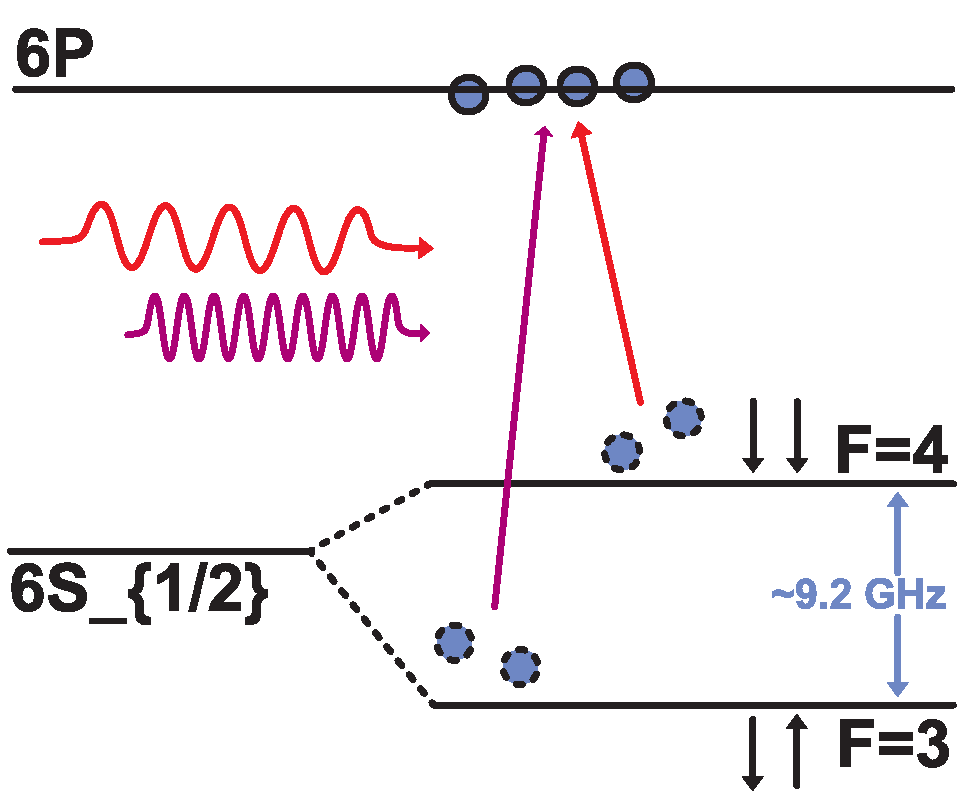
\includegraphics[width=0.9\textwidth]{pdf/CPT/pumping.pdf}}
                \only<2>{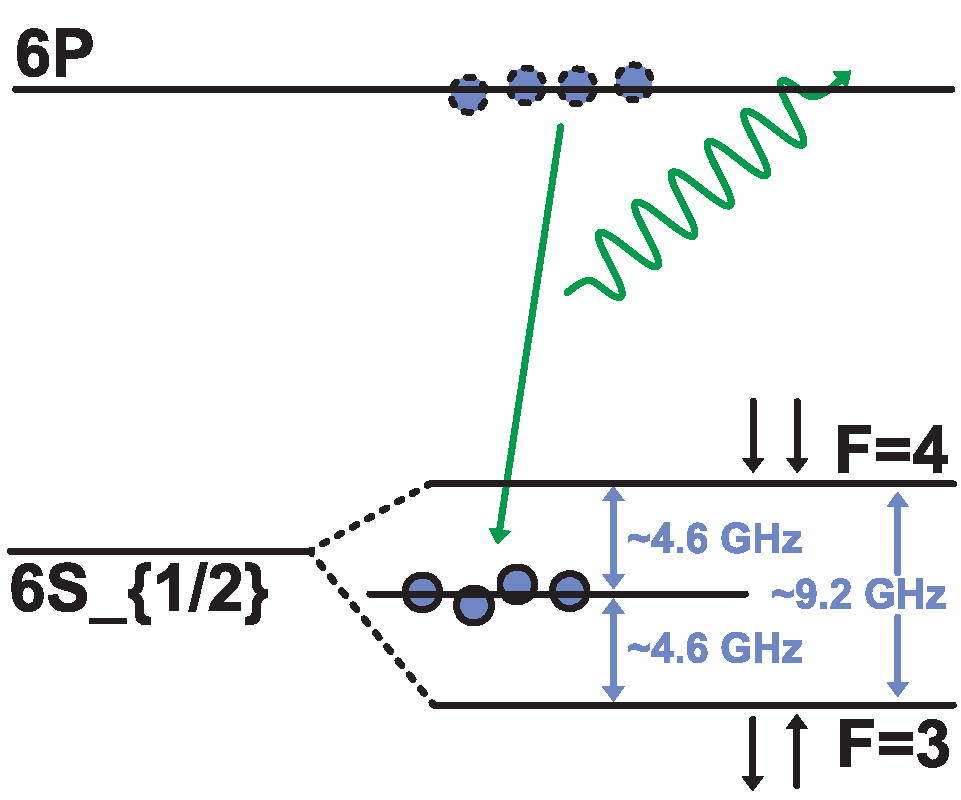
\includegraphics[width=0.9\textwidth]{pdf/CPT/decay.pdf}}
                \only<3>{\includegraphics[width=0.9\textwidth]{pdf/CPT/interrogation.pdf}}
            \end{figure}

        \end{column}

        \begin{column}{0.55\textwidth}

            We can distinguish 3 processes:

            \begin{enumerate}
                \item<1-> \textbf<1>{Optical Pumping (Population Inversion)}
                \item<2-> \textbf<2>{Decay to the dark state (superposition state)}
                \item<3-> \textbf<3>{Optical Pumping (Interrogation)}
            \end{enumerate}

        \end{column}

    \end{columns}

    \vspace{10pt}

    \only<1>{A dual-frequency laser is used to pump the population from both $F=\ket{1}$ and $F=\ket{2}$ to $6P$.}
    \only<2>{
        Because of the particular beat frequency and phase of the laser, the population will (over time) fall into a superposition state.

        \begin{equation}
            \ket{\psi} = \ket{Dark} = \frac{1}{\sqrt{2}} \left( \ket{3} + \ket{4} \right)
        \end{equation}
    }
    \only<3>{
        Being in a superposition state $\ket{\psi}$, the population will not absorb the pumping laser radiation anymore.
        \textbf{Electrons are now trapped.}
    }

\end{frame}



\begin{frame}{Photodetection}

    At the end of the cell, a photodiode is used to measure the intensity of the transmitted radiation.

    \begin{columns}[c, onlytextwidth]

        \begin{column}{0.45\textwidth}

            \begin{figure}
                \centering
                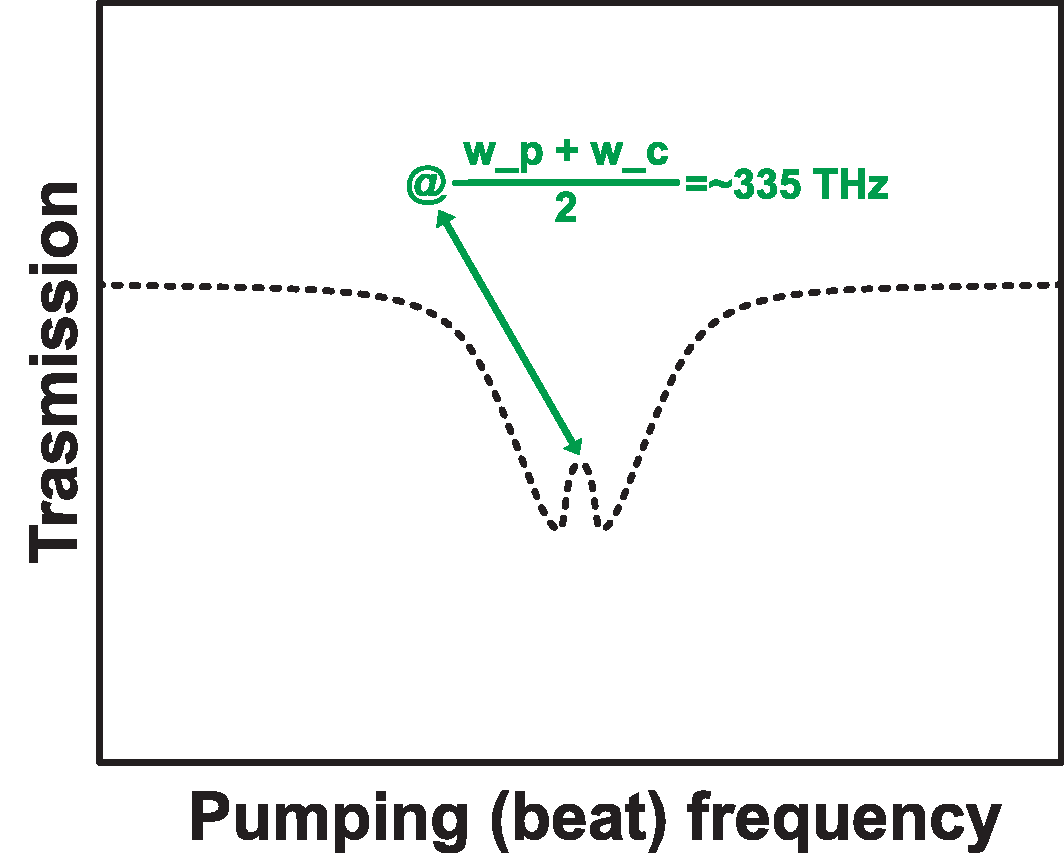
\includegraphics[width=0.9\textwidth]{pdf/CPT-trasmission-curve.pdf}
            \end{figure}

        \end{column}

        \begin{column}{0.55\textwidth}

            \begin{figure}
                \centering
                \includegraphics[width=0.9\textwidth]{pdf/beating-waves.pdf}
            \end{figure}

        \end{column}

    \end{columns}

    \vspace{10pt}

    Our target is to stay at the peak in the middle of the valley in the transmission curve.
    % Notice how that point is associated to a laser frequency of $\approx 4.6 GHz$ in case of $^{133}Cs$.

\end{frame}



\begin{frame}{Complete Physics Package for a CPT-based CSAC}

    \begin{columns}[c, onlytextwidth]

        \begin{column}{0.35\textwidth}

            \begin{figure}
                \centering
                \includegraphics[width=\textwidth]{img/CPT-physics-package-1.png}
            \end{figure}

        \end{column}

        \hfill

        \begin{column}{0.6\textwidth}

            Power consumption\footnotemark[1]: $\approx 10mW$.

            Volume: $\approx 0.35 cm^3$.

            \vspace{10pt}

            \begin{figure}

                \centering
                \only<1>{\includegraphics[width=0.7\textwidth]{img/CPT-physics-package-2.png}}
                \only<2>{
                    \includegraphics[width=0.5\textwidth]{img/CPT-physics-package-3.png}
                    \caption{Microchip SA.45s physics package.}
                }

            \end{figure}

            \footnotetext[1]{The entire package is vacuum sealed to minimize the heating power required (to stabilize).}
            \footnotetext[2]{LCC: Leadless Chip Carrier.}
            \footnotetext[3]{VCSEL: Vertical-Cavity Surface-Emitting Laser.}

        \end{column}

    \end{columns}

\end{frame}



\begin{frame}{Vertical-Cavity Surface-Emitting Laser (VCSEL)}

    % VCSEL, schematics, importance of its stability.

    % Flexibilty in the choice of the optical wavelength (allowance for both Rb and Cs).

    % ~ power consumption (from travaglin @36)

    VCSELs are a type of semiconductor laser diode with laser beam emission perpendicular to the chip surface.

    \begin{figure}
        \centering
        \includegraphics[width=0.6\textwidth]{img/CPT-VCSEL.png}
    \end{figure}

    In CPT-based CSACs, the VCSEL is used as the radiation source:

    \begin{itemize}
        \item Stability in the emitted frequency.
        \item Flexibility in the choice of the optical wavelength.
        \item Low power consumption ($\approx 3mW$).
    \end{itemize}

\end{frame}


\begin{frame}{Design bottleneck}

    CPT-based CSACs partially solve the bottleneck of size and power consumption of the MODR-based CSACs.

    \vspace{10pt}

    Still, we can recognize some area of improvements:

    \begin{itemize}
        \item Working temperature range\footnotemark[1] (currently $\approx [-40; 80]^{\circ}C$).
        \item High sensitivity to temperature and voltage fluctuations.
        \item Short-term frequency stability (currently $\approx 3 \times 10^{-10}@\tau=1s$).
    \end{itemize}

    \footnotetext[1]{Mainly due to degradation in performance of the resonance cell (buffer gas pressure).}

\end{frame}
\section{Control loop}
% Control Loop (differences between the two, from where they start to where they close, freuqency for the various elements)

\begin{frame}{Control loop}

    Close-loop approach to \textbf{lock the LO\footnotemark[1] frequency to the atomic transition}.

    \vspace{10pt}

    \begin{columns}[c, onlytextwidth]

        \begin{column}{0.6\textwidth}

            \begin{figure}
                \centering
                \includegraphics[width=0.9\textwidth]{img/control-loop.png}
                \caption{Control loop block diagram.}
            \end{figure}

        \end{column}

        \begin{column}{0.4\textwidth}

            PI\footnotemark[2] controllers are used to minimize the error between the target and the actual value.

            \vspace{10pt}

            Indispensable targets:

            \begin{itemize}
                \item LO frequency
                \item Laser frequency
                \item Laser temperature
                \item Cell temperature
            \end{itemize}

        \end{column}

    \end{columns}

    \footnotetext[1]{LO: Local Oscillator}
    \footnotetext[2]{PI: Proportional-Integral}

\end{frame}



\begin{frame}{Electronics}

    \begin{columns}[c, onlytextwidth]

        \begin{column}{0.6\textwidth}

            Here are some possible problematic areas:

            \begin{itemize}
                \item Stability in voltage and current provided to VCO and VCSEL (highly sensitive components)
                \item Cross-talk between different control loops
                \item Noise from the electronics
                \item Power consumption ($\approx 10\%$ of the total)
            \end{itemize}

        \end{column}

        \hfill

        \begin{column}{0.35\textwidth}

            \begin{figure}
                \centering
                \includegraphics[width=\textwidth]{img/electronics-CSCA-SA45s.png}
                \caption{CSAC SA.45s from Microchip.}
            \end{figure}

        \end{column}

    \end{columns}

\end{frame}
\section{Local Oscillator}

\begin{frame}{Local Oscillator}

    Normally, the local oscillator in a CSAC is a quartz crystal oscillator (XO).

    There exist many versions of the XO, differentiated based on the environmental correction type applied to enhance stability:

    \begin{itemize}
        \item \textbf{TCXO}: Temperature Compensated Crystal Oscillator
        \item \textbf{MCXO}: Microcomputer Compensated Crystal Oscillator
        \item \textbf{OCXO}: Oven Controlled Crystal Oscillator
    \end{itemize}

\end{frame}



\begin{frame}{Quartz Crystal Oscillator}

    \textbf{At short time scales, the quartz crystal oscillator is the main source of instability} in a CSAC due to its phase noise.

    \begin{columns}[c, onlytextwidth]

        \begin{column}{0.6\textwidth}

            Here are some other problematic areas:

            \begin{itemize}
                \item High temperature sensitivity
                \item Power consumption (due to thermal control to enhance stability)
                \item Aging and frequency drift
            \end{itemize}

        \end{column}

        \begin{column}{0.4\textwidth}

            \begin{figure}
                \centering
                \includegraphics[width=0.9\textwidth]{img/thin-local-oscillator.png}
                \caption{Resonator with 2-mm quartz thickness\footnotemark[1].}
            \end{figure}

        \end{column}

    \end{columns}

    In the end, the choice of a local oscillator is a trade-off between stability and power consumption.

    \footnotetext[1]{Photograph taken using Scanning Electron Microscope (SEM) technique.}

\end{frame}

\appendix

\begin{frame}[standout]
    Extra slides
\end{frame}



\begin{frame}{Reference cell (buffer gas \& cell size)}

    Collision with untreated walls of the reference cell can depolarize the spin of electrons, forcing them to return to the ground state.

    To avoid this, we can either \textbf{add a buffer gas to reduce the number of collisions} composed of a mixture of $N_2$, $Ne$, $Ar$, and $He$ or \textbf{reduce the mean free path of atoms (larger cell)}.

    \begin{columns}[c, onlytextwidth]

        \begin{column}{0.5\textwidth}

            \begin{figure}
                \centering
                \includegraphics[width=0.7\textwidth]{img/extra-cell-pressure.png}
                \caption{Result of diffusion to the walls (red dotted line) and buffer gas collisions (dashed blue line).}
            \end{figure}

        \end{column}

        \begin{column}{0.5\textwidth}

            \begin{figure}
                \centering
                \includegraphics[width=0.7\textwidth]{img/extra-cell-size.png}
                \caption{Cell with a $100 kPa$ nitrogen buffer gas (red) or a paraffin wall coating (black).}
            \end{figure}

        \end{column}

    \end{columns}

    \footnotetext{FWHM: Full Width at Half Maximum}

\end{frame}



\begin{frame}{Quantum levels of $^{133}Cs$ and $^{87}Rb$}

    \begin{columns}[c, onlytextwidth]

        \begin{column}{0.5\textwidth}

            \begin{figure}
                \centering
                \includegraphics[height=0.7\textheight]{img/levels-Rubidium.png}
                \caption{$^{87}Rb$ quantum level.}
            \end{figure}

        \end{column}

        \begin{column}{0.5\textwidth}

            \begin{figure}
                \centering
                \includegraphics[height=0.7\textheight]{img/levels-Caesium.png}
                \caption{$^{133}Cs$ quantum level.}
            \end{figure}

        \end{column}

    \end{columns}

\end{frame}



\begin{frame}{Zeeman effect and c-field for clock calibration}

    The Zeeman effect is the splitting of atomic energy levels due to the presence of an external magnetic field.

    \begin{figure}
        \centering
        \includegraphics[width=0.5\textwidth]{img/extra-zeeman-splitting.png}
        \caption{$^{133}Cs$ $6S_{1/2}$ (ground) level hyperfine structure in an external magnetic field}
    \end{figure}

    A fine calibration of the clock can be done by applying a c-field (controlled magnetic field) to the reference cell.

\end{frame}


\begin{frame}[allowframebreaks]{References}
    \nocite{*}
    \bibliography{references}
\end{frame}

\begin{frame}[standout]
    Questions?
\end{frame}

\begin{frame}[standout]
    Thank you!
\end{frame}

\end{document}